\documentclass[12pt,a4paper]{article}

% ---------- Page layout ----------
\usepackage[a4paper,margin=2.5cm]{geometry}
\usepackage{setspace}
\onehalfspacing
\setlength{\parindent}{0pt}
\setlength{\parskip}{0.75em}

% ---------- Tables and figures ----------
\usepackage{graphicx}
% Figures are generated into the repository's outputs directory by
% scripts/plot_thesis_figures.py rather than kept beside this file.
\graphicspath{{../../outputs/figures/}}
\usepackage{booktabs}
\usepackage{threeparttable}
\usepackage{caption}
\usepackage{subcaption}
\usepackage{float}
\usepackage{array}
\usepackage{longtable}
\usepackage{tabularx}
\usepackage{array}

% ---------- Math and symbols ----------
\usepackage{amsmath}
\usepackage{amssymb}

% ---------- References ----------
\usepackage[round,authoryear]{natbib}
\bibliographystyle{apalike}

% ---------- Links ----------
\usepackage{xcolor}
\usepackage[
    colorlinks=true,
    linkcolor=black,
    citecolor=blue,
    urlcolor=blue
]{hyperref}

% ---------- Thesis metadata ----------
\newcommand{\thesistitle}{War Signals and Defense Equity Risk: Physical Air-Attack Intensity versus Multilingual News Narratives}
\newcommand{\thesisauthor}{Khrystyna Kateryna Valenia}
\newcommand{\thesisdate}{August 2026}

\begin{document}

% ---------- Title page ----------
\begin{titlepage}
    \centering
    \vspace*{2cm}

    {\LARGE\thesistitle\par}
    \vspace{1cm}

    {\large \thesisauthor\par}
    \vspace{0.5cm}
    {\large \thesisdate\par}
    \vspace{1cm}

    \begin{abstract}
    \noindent
    This thesis studies whether daily information from the Russia--Ukraine war improves forecasts of defense-equity returns and volatility. The analysis combines official Bloomberg defense-equity indices, Ukrainian Air Force data on Russian air attacks, and multilingual GDELT news data classified by the country and ownership of the publishing outlet into Ukrainian, Russian state, Russian independent, Western, and native-English source groups. The main outcome is the Bloomberg World Large, Mid and Small Aerospace \& Defense Total Return Index (WAERLST), with the Bloomberg Europe Defense Select Total Return Index (BSHIELDT) and the iShares U.S. Aerospace \& Defense ETF (ITA) used as robustness outcomes. The empirical strategy is predictive rather than causal: information available through day $t$ is used to forecast defense-equity outcomes on future trading days. The thesis compares financial-only benchmarks with models that add physical attack variables, news variables, and narrative-gap variables in an out-of-sample expanding-window design, and evaluates them using out-of-sample $R^2$, tests appropriate to nested and non-nested comparisons, and a false-discovery-rate correction across the full grid of specifications. The main result is conservative: war-specific physical and news variables do not provide robust incremental predictive power beyond simple financial benchmarks, for returns or for volatility.
    \end{abstract}
\end{titlepage}

\newpage

\section{Introduction}

Russia's full-scale invasion of Ukraine has turned geopolitical risk into a daily financial-market concern. The war combines military escalation, sanctions, energy shocks, changes in defense budgets, and a continuous flow of news about attacks on Ukrainian cities and infrastructure. For investors, such information may matter not only because war increases aggregate uncertainty, but also because it can change expectations about future demand for aerospace and defense firms. This makes the defense sector an unusual setting: geopolitical shocks that are negative for broad markets may contain positive demand news for firms producing military equipment, air-defense systems, drones, missiles, aircraft, electronics, and related services.

This thesis asks whether daily war information helps forecast defense-equity returns and volatility. The central research question is: do physical Russian air-attack intensity and multilingual news narratives provide incremental out-of-sample predictive information for defense-equity returns and volatility? The question is deliberately predictive rather than causal. The goal is not to claim that a given attack or article causes a stock-price movement. Instead, the thesis asks whether information available to investors by the end of day $t$ improves forecasts of defense-equity outcomes on future trading days, relative to models that use only standard financial controls.

The distinction between correlation, causality, and predictability is important for this topic. Wars create many simultaneous shocks: military events, political speeches, sanctions, procurement announcements, humanitarian events, energy-market movements, and changes in investor risk appetite. These channels make causal identification difficult without a separate research design. A forecasting design is more appropriate for the scope of this thesis because it evaluates whether a clearly defined information set improves prediction in real time. This also sets a high empirical standard, since equity-return predictability is difficult to establish out of sample \citep{goyal2008equity}.

The first challenge is to define a reliable defense-equity outcome. The primary financial target is the Bloomberg World Large, Mid and Small Aerospace \& Defense Total Return Index, hereafter WAERLST. This index provides a global defense-equity outcome and avoids the main limitation of using only a U.S. exchange-traded fund. The Bloomberg Europe Defense Select Total Return Index, hereafter BSHIELDT, is used as a European robustness outcome, while ITA, the iShares U.S. Aerospace \& Defense ETF, is retained as a U.S. traded-proxy robustness outcome. Using all three outcomes separates the global question from two robustness perspectives: European defense exposure and U.S. defense exposure.

The second challenge is to measure physical war intensity without introducing look-ahead bias. Russian air attacks often begin at night, cross calendar dates, and are officially reported only after the attack window closes. A naive date assignment could place information into the model before it was available to investors. To avoid this problem, the thesis uses a market-information date that reflects when verified attack information could enter the market's information set. The physical variables include total weapons launched, weapons destroyed, interception rates, weapon composition, attack-surprise measures, and large-attack indicators.

A related point concerns what the absence of an attack record means. The Ukrainian Air Force began publishing daily tallies in late September 2022, which is not the date on which air attacks began. Treating every earlier date as a day of zero attacks would be correct for the years before the full-scale invasion and clearly false for the months immediately after it. Section~\ref{sec:attacks} sets out the three-part treatment that this requires.

The third challenge is to separate realized physical intensity from media narratives. News coverage can amplify, interpret, or selectively emphasize military events. It may therefore contain information not captured by physical counts alone. At the same time, media attention is not a neutral mirror of the battlefield: Ukrainian, Russian, Western, and other sources may frame the same attack differently. The thesis addresses this issue using multilingual GDELT news data and a source-group classification built on the identity of the publishing outlet rather than on the subject matter of an article. Because outlets in this conflict routinely publish in a language other than that of their own country, and because many Ukrainian outlets publish in Russian, the classifier resolves country before language, and it separates Russian state-controlled outlets from Russian independent and exile outlets. This design makes it possible to compare physical attacks, raw news attention, tone, and cross-source narrative differences within the same empirical framework.

The fourth challenge is empirical evaluation. The thesis compares several information sets: financial controls only, financial controls plus physical attacks, financial controls plus news narratives, financial controls plus both attacks and news, and a final set adding narrative gaps across source groups. These comparisons are made using an out-of-sample time-series design, not random train-test splits. All models are evaluated on identical forecast dates and on identical observations, and any preprocessing or estimated feature construction is designed to use only information available before the forecast. This design is meant to ensure that any observed improvement reflects predictive content rather than future information, sample-selection differences, or full-sample normalization. Because the design produces a large grid of specifications, the thesis also applies a false-discovery-rate correction across that grid, so that the number of apparently significant cells is not itself a product of the number of cells examined.

The empirical contribution of the thesis is to compare two layers of war information that are often studied separately. The physical layer measures what happened: the scale and composition of Russian air attacks and interception outcomes. The narrative layer measures how the war was reported: the amount and tone of multilingual news coverage across source groups, and the differences between them. The thesis asks whether one layer dominates the other, whether they are complementary, and whether the combination improves forecasts of returns or volatility beyond standard financial variables.

The empirical results provide little evidence of incremental predictability from war-specific variables. Across 144 return specifications, spanning three outcomes, two horizons, two samples, and five information sets, 16 produce a positive out-of-sample $R^2$ and none survives the false-discovery-rate correction. Models that use no war variables at all win eight of the twelve outcome-horizon-sample cells. At the one-day horizon the combined physical-and-news set does improve on the historical mean for WAERLST, by 1.8 percent in mean absolute error, but the improvement is not statistically distinguishable from zero once the size of the grid is accounted for, and it reverses at the five-day horizon. The volatility results are also conservative: standard GARCH-family benchmarks are not improved upon by war-augmented specifications under the QLIKE loss, and where the difference is statistically detectable the augmented model is worse. Overall, the evidence suggests that daily attack and news signals are either quickly incorporated into defense-equity prices, too noisy at the daily frequency, or dominated by broader financial dynamics.

This thesis is related to a broad literature on uncertainty measurement and financial markets. \citet{baker2016epu} show that newspaper-based measures can capture economic policy uncertainty and are associated with stock-price volatility, investment, and employment. \citet{caldara2022gpr} construct a news-based geopolitical-risk index and show that geopolitical risk is associated with weaker real activity, lower investment, and downside risks. Their distinction between geopolitical threats and realized adverse events is especially useful here, because this thesis separately measures realized air-attack intensity and news narratives about the war.

The thesis also builds on research showing that media content can matter for asset prices. \citet{tetlock2007media} finds that negative media content predicts short-run market movements, while \citet{loughran2011textual} shows that textual measures require careful domain-specific interpretation in financial applications. These papers motivate the use of news attention and tone as possible predictors, but they also caution against treating automated textual measures as perfect sentiment indicators. In this thesis, GDELT-based news measures are therefore interpreted as scalable proxies for attention and tone, not as complete measures of investor beliefs.

A closely related contribution is \citet{bondarenko2024perceptions}, who construct geopolitical-risk indicators separately from local-language and English-language sources and find that the two behave differently: local-language risk shocks move Russian macroeconomic aggregates while English-language shocks do not. That result motivates the source-group design used here. If the measured effect of the same underlying event depends on whose newspapers are read, then a study that draws its national series from a single language population cannot address the question at all.

The closest literature studies defense equities during periods of geopolitical stress. \citet{apergis2018defense} examine whether geopolitical risk predicts returns and volatility of leading defense companies. \citet{zhang2022race} study co-movements between daily geopolitical risk and the returns and volatility of global defense and aerospace firms, finding strong patterns around the Russia--Ukraine war and interpreting them as evidence of a possible ``flight-to-arms'' mechanism. \citet{covachev2024europe} use an event-study design and report positive abnormal returns for European defense stocks after the start of the Russia--Ukraine war. \citet{klomp2025hamas} similarly finds a positive relationship between Hamas--Israel conflict intensity and U.S. defense-industry ETF returns.

This thesis differs from much of the existing defense-stock literature in three ways. First, it uses daily physical attack measures rather than relying only on aggregate geopolitical-risk indices or major event dates. Second, it explicitly separates physical war intensity from multilingual media attention and source-group narratives, and does so by publisher rather than by subject. Third, it evaluates predictive performance out of sample, asking whether each information layer improves forecasts relative to financial benchmarks, and bounds the resulting null with tests and corrections appropriate to the size of the specification grid. In this sense, the thesis contributes to the literature by shifting the focus from whether defense stocks react around major war events to whether daily war signals can help forecast defense-equity returns and volatility in a reproducible forecasting framework.

\section{Data and Identification Strategy}

\subsection{Overview}

The empirical design combines three daily information sets: financial-market data, physical air-attack data, and multilingual news data. The financial data define the defense-equity outcomes to be forecast. The attack data measure the physical intensity and composition of Russian air attacks against Ukraine. The news data measure attention and tone across source groups. The final modeling dataset aligns these information sets by date so that information available through day $t$ predicts market outcomes on future trading days.

\subsection{Financial Outcomes}

The primary financial outcome is the official Bloomberg WAERLST index. WAERLST is denominated in U.S. dollars and observed daily from 1 January 2020 to 30 June 2026 in the Bloomberg export used for this thesis. The daily return is defined as:

\begin{equation}
r^{W}_{t} = 100 \times \ln\left(\frac{P^{W}_{t}}{P^{W}_{t-1}}\right),
\end{equation}

where $P^{W}_{t}$ is the WAERLST closing index level on day $t$. Returns are expressed in percent so that forecast errors are interpretable in daily percentage-point units.

The main robustness outcomes are official BSHIELDT returns and ITA returns. BSHIELDT is denominated in euros and provides a European defense-equity comparison. ITA is a liquid U.S. aerospace and defense ETF and is useful because it is traded, reproducible, and U.S.-focused. Using all three outcomes separates the global question from two robustness perspectives: European defense exposure and U.S. defense exposure.

The financial controls include broad equity-market returns, volatility, energy prices, exchange rates, and lagged defense-equity variables. The broad-market controls are included because defense equities may move with aggregate risk appetite rather than war-specific information. The volatility controls are included because geopolitical news may coincide with changes in market-wide uncertainty. The return controls also reduce the risk that attack or news variables are simply proxying for persistent financial conditions.

\subsection{Physical Attack Variables}
\label{sec:attacks}

The physical attack dataset is based on Ukrainian Air Force records of Russian air attacks. The raw file contains 3,812 attack-level records from 29 September 2022 to 21 June 2026. The processing pipeline aggregates these records to 809 unique market-information dates. Across the raw records, 102,396 weapons were launched and 76,126 were intercepted or destroyed, implying an aggregate interception rate of approximately 74.3 percent. UAVs dominate the sample, representing about 94.8 percent of all launched weapons.

The key timing rule is the market-information date:

\begin{equation}
\text{market\_info\_date} =
\max(\text{attack\_date}, \text{time\_end\_date}).
\end{equation}

This rule assigns an overnight attack to the day on which the attack ended and the verified count could plausibly become public. For example, an attack wave beginning late on day $t-1$ and ending in the morning of day $t$ is assigned to day $t$, not day $t-1$. This avoids look-ahead bias in the forecasting exercise.

The main physical variables are total weapons launched, total weapons destroyed, interception rate, weapon diversity, and category-specific launch counts. Weapon categories include UAVs, cruise missiles, ballistic missiles, reconnaissance UAVs, loitering munitions, guided bombs, and other weapons. War intensity is measured as:

\begin{equation}
\text{Attack intensity}_{t} = \ln(1 + \text{weapons launched}_{t}).
\end{equation}

The logarithmic transformation reduces the influence of extreme attack waves while preserving the ordering of attack intensity.

The model also includes surprise-style attack measures. These variables compare recent attack intensity with rolling historical expectations, for example using seven-day, thirty-day, and ninety-day windows. The purpose is to distinguish routine wartime activity from unexpectedly large or intense attack days. In the forecasting interpretation, such variables ask whether unusually large attacks contain more market-relevant information than the level of attacks alone.

The attack series begins when the Ukrainian Air Force began publishing systematic daily tallies, which is not the date on which attacks began. The absence of a record therefore means different things at different times, and the sample is treated in three parts.

Before 24 February 2022 the physical variables are set to zero. No Russian mass air campaign against Ukrainian cities existed in this period, and the earlier phase of the conflict was fought with artillery and ground forces. This is a substantive assumption rather than an observation, and it is also what each formula returns on an all-zero history: no weapons, no composition, and no surprise relative to a rolling mean of nothing.

Between 24 February 2022 and 28 September 2022 the physical variables are treated as unobserved. This window contains the cruise-missile campaign against Kyiv, Vinnytsia, Kremenchuk, and Odesa; those attacks occurred and were not tallied in this format. Coding them as zero would assert that no air attacks took place during the invasion of Ukraine, and would do so across the period in which defense equities repriced most sharply, which would teach any model that attack intensity was nil precisely when the market moved most. These 149 trading days are therefore excluded from every specification, including those that use no physical variables, so that the information sets are compared on identical observations.

From 29 September 2022 onward the variables are observed. Trading days inside this window with no published attack wave are genuine zeros and are treated as such; 809 of the 931 trading days in the window carry a Ukrainian Air Force record.

\subsection{News and Narrative Variables}
\label{sec:news}

The news dataset is constructed from GDELT GKG 2.0, a large-scale global database designed to measure events, locations, and tone from news sources \citep{leetaru2013gdelt}. The extraction covers 18 February 2015 to 20 May 2026, or 4,027 days, which is 98 percent of the calendar in that span; the missing days are gaps in the GDELT archive itself. Coverage begins well before the full-scale invasion so that the news series are observed across quiet periods, the 2021--2022 build-up, and the war itself, rather than only during the conflict.

News sources are classified by the identity of the outlet that published an article, not by the country an article mentions. The distinction is essential rather than technical. Classifying by subject would place a Western wire report about Russia in the Russian group, so that all national series would be drawn from a single English-language population and would differ only in topic; the question of whether the perception carried by different media matters cannot be answered by a classifier of that kind.

The classifier applies four tiers in order. Syndication platforms with no newsroom of their own are excluded first, because they carry large volume but no editorial voice. A curated register of the highest-volume outlets is applied next, recording country and, for Russian outlets, state control as against independent or exile ownership. Country top-level domains are applied third. Source language is applied last and only where country remains unknown. Country resolves before language because many Ukrainian outlets publish heavily in Russian, so a language-first rule would file them as Russian media and manufacture agreement between the two groups; Section~\ref{sec:classcheck} reports what such a rule costs in practice.

Five source groups enter the tests: Ukrainian, Russian state, Russian independent, Western, and native-English. Russian outlets outside the register are retained as a residual group that is reported but not tested, so that unclassified Russian volume remains visible rather than hidden inside another series.

The daily news variables measure both attention and tone. Attention is each group's conflict-related coverage as a share of its own total output rather than as a raw count, because GDELT source coverage drifts substantially over eleven years and a count series would show that drift as a common trend in every group at once. Tone is the average GDELT tone score for articles in a given group and day. Because GDELT tone is a scalable automated measure, it is interpreted as an indicator of article negativity or positivity rather than a perfect measure of investor sentiment. This interpretation follows the broader caution in financial textual analysis that dictionaries and automated textual scores may behave differently across domains \citep{loughran2011textual}.

The narrative-gap variables compare tone across source groups. The main gaps are:

\begin{align}
\text{UA--West gap}_{t} &= \text{Tone}^{UA}_{t} - \text{Tone}^{West}_{t}, \\
\text{RU--West gap}_{t} &= \text{Tone}^{RU}_{t} - \text{Tone}^{West}_{t}, \\
\text{UA--RU gap}_{t} &= \text{Tone}^{UA}_{t} - \text{Tone}^{RU}_{t}, \\
\text{State--independent gap}_{t} &= \text{Tone}^{RU\,state}_{t} - \text{Tone}^{RU\,indep}_{t}.
\end{align}

These variables are designed to measure whether differences in wartime framing contain predictive information beyond the volume of news. For example, a strongly negative Ukrainian-versus-Western tone gap may indicate that local sources describe the war as more severe than Western sources on the same day. The fourth gap isolates ownership while holding country and language fixed.

\subsection{Forecasting Design}

The empirical strategy is an out-of-sample forecasting horse race. Let $y_{t+h}$ denote the defense-equity outcome over horizon $h$, where $h=1$ or $h=5$ trading days. The general predictive specification can be written as:

\begin{equation}
y_{t+h} = \alpha + \beta'F_t + \gamma'P_t + \delta'N_t + \theta'G_t + \varepsilon_{t+h},
\end{equation}

where $F_t$ contains financial controls, $P_t$ contains physical attack variables, $N_t$ contains news attention and tone variables, and $G_t$ contains narrative-gap variables. All variables on the right-hand side are dated so that they are available before the forecast target is realized.

The main information sets are defined as follows:

\begin{table}[H]
\centering
\caption{Information sets used in the forecasting horse race}
\label{tab:info_sets}
\begin{threeparttable}
\begin{tabular}{p{2cm} p{4cm} p{7cm}}
\toprule
Code & Name & Content \\
\midrule
F & Financial baseline & Lagged defense-equity returns and volatility proxies, broad equity-market returns, VIX, energy prices, exchange rates, long rates, and regime controls. \\
P & Physical attacks & F plus Russian air-attack variables, including launched weapons, destroyed weapons, interception rate, weapon composition, attack surprises, and large-attack indicators. \\
N & News & F plus news attention and tone variables by source group. \\
PN & Physical + news & F plus physical attack variables and news variables. \\
PNG & Physical + news + gaps & PN plus narrative-gap variables comparing Ukrainian, Russian state, Russian independent, and Western tone. \\
\bottomrule
\end{tabular}
\begin{tablenotes}
\small
\item Notes: The model matrix contains 21 features in F, 62 in P, 31 in N, 72 in PN, and 76 in PNG.
\end{tablenotes}
\end{threeparttable}
\end{table}

The out-of-sample design uses an expanding training window. The last quarter of the modeling sample is held out for testing. Models are estimated on the initial training period, forecasts are generated for the next block of test observations, and the training window is then expanded and the model refit at a fixed cadence. This procedure respects the time ordering of the data and avoids random train-test splits, which would be inappropriate for a forecasting problem.

All models are estimated on trading days. Defense-equity returns exist only on days the relevant market is open, and carrying a realized return forward across a weekend would repeat the same outcome on several dates while the attack and news variables differ across them; that would ask a model to predict one identical value from several distinct inputs and would distort every out-of-sample statistic computed from it.

Two samples are reported throughout. The full sample runs from February 2015 and carries the pre-war period as substantive zeros in the physical block. The measured sample is restricted to 29 September 2022 onward, so that every physical observation is a counted one. Reporting both makes the cost of the zero-fill assumption visible rather than assumed away. Within each sample, all information sets are estimated on one common set of observations, so that the comparison between them is not confounded by differences in coverage.

\subsection{Models and Evaluation}

The return-forecast baselines are the historical mean, an autoregressive AR(1) model, and ridge regression. The historical mean is a difficult benchmark for daily return prediction because equity returns are noisy and close to unpredictable at short horizons. The AR(1) model tests whether return persistence matters; at the five-day horizon its predictor is the most recent fully realized five-day return, because overlapping windows would otherwise place part of the forecast target inside the predictor. Ridge regression tests whether the information sets improve forecasts in a linear model, with shrinkage where many predictors are included.

The main machine-learning model is XGBoost, a gradient-boosted tree algorithm \citep{chen2016xgboost}. XGBoost is useful here because it can capture nonlinearities and interactions between attacks, news, and financial variables while handling missing predictor values internally. Hyperparameters are held fixed and identical across information sets. This is deliberate: a comparison in which one information set receives tuning that the others do not is not a comparison of information sets. Where feature importance is discussed, SHAP values would be the natural tool \citep{lundberg2017shap}, but Section~\ref{sec:mlinterp} explains why that interpretation is treated as secondary here.

Volatility forecasts are evaluated with GARCH-family models. The benchmark specifications include GARCH, GJR-GARCH, and EGARCH, following the standard volatility-modeling literature \citep{bollerslev1986garch,glosten1993gjr,nelson1991egarch}. Because the available financial data are daily closing levels rather than intraday prices, realized volatility is proxied using squared returns or sums of squared returns over the forecast horizon.

The war variables enter the volatility exercise through a heterogeneous autoregressive specification, HAR-RV-X: log realized variance is regressed on its own one-, five-, and twenty-two-day averages \citep{corsi2009har}, and the war blocks are then added to that regression. Exogenous regressors cannot be placed in the variance equation of a standard GARCH model directly, and this is the conventional way to admit them to a volatility forecast; it also has the practical advantage that the exogenous block demonstrably enters the fitted model rather than being carried alongside it without effect.

The loss function for volatility is QLIKE, which is commonly used when evaluating volatility forecasts because it is robust to noise in the volatility proxy \citep{patton2011volatility}.

Forecast accuracy is evaluated using mean absolute error, root mean squared error, directional accuracy, and the Campbell--Thompson out-of-sample $R^2$ \citep{campbell2008predicting}, defined as one minus the ratio of the model's mean squared forecast error to that of the historical-mean benchmark. Volatility forecasts are evaluated using QLIKE, mean absolute error, root mean squared error, and bias.

Formal comparisons follow the nesting structure of the design. Each information set contains the one before it, so a comparison between an information set and the financial baseline is a nested comparison, and the Diebold--Mariano statistic \citep{diebold1995predictive} is not valid there; the Clark--West test is used instead \citep{clark2007nested}. Diebold--Mariano is used where the models being compared are genuinely non-nested, as when a GARCH-family model is compared with a heterogeneous autoregressive specification. Because the design produces a large grid of specifications, $p$-values are corrected across the whole grid using the Benjamini--Hochberg false-discovery-rate procedure \citep{benjamini1995fdr}. The interpretation is always predictive: a lower forecast error means that the information set was useful for prediction in the test period, not that the predictors caused the market outcome.

\subsection{Identification Challenges and Interpretation}

The empirical strategy is designed for forecasting, not causal identification. Attacks are not randomly assigned, news coverage responds to both battlefield events and market conditions, and defense-equity returns are affected by many global shocks. Even if attack or news variables improve forecast accuracy, the result should be interpreted as evidence that these variables contain information useful for prediction, not as evidence that attacks or articles mechanically caused returns.

The main identification challenge is information timing. The pipeline addresses this challenge by assigning physical attacks to a market-information date, lagging predictors before forecasting, and evaluating models only on future trading outcomes. The second challenge is avoiding overfitting in a small daily sample. The pipeline addresses this through out-of-sample testing, expanding-window validation, hyperparameters held fixed across information sets, comparisons against simple benchmarks, and a false-discovery-rate correction across the specification grid. The third challenge is measurement error in news and source classification. The pipeline addresses this by classifying on the publisher rather than the subject, by validating the classifier against an independent external source, and by re-running the central comparison under alternative classification rules; Section~\ref{sec:classcheck} reports both.

\section{Descriptive Statistics}

\subsection{Financial Outcomes}

The official WAERLST and BSHIELDT files provide complete weekday coverage from 1 January 2020 to 30 June 2026. WAERLST has 1,695 daily observations, 100 percent non-missing price coverage, and no zero-volume days in the Bloomberg export. BSHIELDT also has 1,695 daily observations and 100 percent non-missing price coverage, but it contains several zero-volume European holiday dates. These holiday dates should be handled carefully in robustness analysis so that non-trading days do not create artificial zero returns.

\begin{table}[H]
\centering
\caption{Official Bloomberg defense-equity index data}
\label{tab:financial_data}
\begin{threeparttable}
\begin{tabular}{lrrrrr}
\toprule
Index & Currency & Start date & End date & Price coverage & Full-period daily std. \\
\midrule
WAERLST & USD & 2020-01-01 & 2026-06-30 & 100.0\% & 1.518\% \\
BSHIELDT & EUR & 2020-01-01 & 2026-06-30 & 100.0\% & 1.770\% \\
\bottomrule
\end{tabular}
\begin{tablenotes}
\small
\item Notes: WAERLST is the Bloomberg World Large, Mid and Small Aerospace \& Defense Total Return Index and is the main outcome. BSHIELDT is the Bloomberg Europe Defense Select Total Return Index and is used for European robustness. Daily standard deviations are computed from log returns in percent over the full available Bloomberg sample.
\end{tablenotes}
\end{threeparttable}
\end{table}

During the model-window period beginning on 29 September 2022, WAERLST daily returns have a mean of 0.108 percent and a standard deviation of 1.056 percent. BSHIELDT daily returns have a mean of 0.148 percent and a standard deviation of 1.445 percent over the same window. The return correlation between WAERLST and BSHIELDT over the full period is approximately 0.756, which indicates that the global and European defense indices are strongly related but not identical.

\subsection{Attack and News Variables}

The attack data show that Russian air attacks became a frequent and high-intensity feature of the war. On days with a recorded attack, an average of about 127 weapons were launched, with a standard deviation of about 144 and a maximum close to 982. The interception rate averages about 0.74 across the sample. These statistics show why both the level and composition of attacks may matter: the distribution is highly skewed, with a small number of very large attack waves.

The news data contain broad daily coverage of the war across the whole 2015--2026 span. Volume differs substantially across source groups, which is one reason attention is measured as a share of a group's own output rather than as a count: the Western group publishes a median of about 7,600 conflict-related articles a day and the Russian independent group about 390. Tone differs as well. Ukrainian and Russian independent coverage is more negative on average, at about $-2.39$ and $-2.31$, than Western coverage at about $-1.80$ or Russian state coverage at about $-1.78$.

Panel B of Table~\ref{tab:summary_statistics} reports how the indicators move together over the full sample, which bears directly on whether the two layers are worth separating. They are. Attack intensity correlates with the narrative indicators at between 0.23 and 0.58 in absolute value, so the physical and media layers are related without being substitutes for one another. The pattern within that range is itself informative: attack intensity moves with Russian state attention at 0.58 and against Ukrainian attention at $-0.35$, so the same battlefield activity is reflected very differently depending on which press is doing the reflecting. Ukrainian and Western attention are the most closely related pair at 0.66, and the three tone series move together at 0.45 to 0.50, which is what one would expect of measures that respond to the same events with different emphasis.

The published geopolitical risk index sits closest to Western attention at 0.46 and to attack intensity at 0.42, and is almost unrelated to Ukrainian attention at 0.07. That is consistent with a global index built largely from Anglophone coverage, and it is one reason a source-group design can say something an aggregate index cannot.

The Russian independent group is much the smallest, and it is small for reasons connected to what it measures. Several of its constituent outlets were liquidated, blocked, or relocated abroad during the sample, so its volume falls sharply across the very event being studied. Results that depend specifically on that group are correspondingly less well determined than results resting on the larger groups.

\begin{table}[H]
\centering
\caption{Main variable definitions}
\label{tab:variables}
\begin{threeparttable}
\begin{tabular}{p{3.5cm} p{2.8cm} p{7.3cm}}
\toprule
Variable & Unit & Definition \\
\midrule
$r^{W}_{t}$ & percent & Daily log return on WAERLST, computed as $100 \times \ln(P_t/P_{t-1})$. \\
$r^{B}_{t}$ & percent & Daily log return on BSHIELDT, used as European robustness outcome. \\
$r^{ITA}_{t}$ & percent & Daily log return on ITA, used as U.S. robustness outcome. \\
Attack intensity & log count & $\ln(1+\text{total weapons launched})$ on the market-information date. \\
Interception rate & ratio & Total weapons destroyed divided by total weapons launched. \\
Weapon composition & counts/shares & Counts or shares of launched weapons by category: UAVs, cruise missiles, ballistic missiles, reconnaissance UAVs, loitering munitions, guided bombs, and other weapons. \\
News attention & count & Number of GDELT articles in a given day, query category, and source group. \\
Tone & score & Average GDELT tone for articles in a given source group and day. More negative values indicate more negative news language. \\
Narrative gap & score difference & Difference between average tone in two source groups, for example Ukrainian tone minus Western tone. \\
\bottomrule
\end{tabular}
\begin{tablenotes}
\small
\item Notes: The empirical tables use these model-matrix variable concepts. Financial returns are measured in percent. Attack and news variables are dated before the financial target to avoid look-ahead bias.
\end{tablenotes}
\end{threeparttable}
\end{table}

\begin{table}[H]
\centering
\caption{Descriptive statistics and correlations}
\label{tab:summary_statistics}
\begin{threeparttable}

\footnotesize
\textit{Panel A. Summary statistics for selected modeling variables}

\begin{tabular}{lrrrrr}
\toprule
Variable & Mean & Std. dev. & Min & Max & N \\
\midrule
WAERLST return, model window & 0.108 & 1.056 & -8.655 & 4.858 & 978 \\
BSHIELDT return, model window & 0.148 & 1.445 & -8.552 & 10.131 & 978 \\
Weapons launched, attack days & 126.6 & 144.2 & 1.0 & 982.0 & 809 \\
Interception rate & 0.743 & --- & 0.000 & 1.000 & 809 \\
Ukrainian articles per day (median) & 4988 & --- & --- & --- & 4027 \\
Russian state articles per day (median) & 2912 & --- & --- & --- & 4027 \\
Russian independent articles per day (median) & 387 & --- & --- & --- & 4027 \\
Western articles per day (median) & 7605 & --- & --- & --- & 4027 \\
Ukrainian tone & -2.390 & --- & --- & --- & 4027 \\
Russian state tone & -1.778 & --- & --- & --- & 4027 \\
Russian independent tone & -2.312 & --- & --- & --- & 4027 \\
Western tone & -1.802 & --- & --- & --- & 4027 \\
\bottomrule
\end{tabular}

\vspace{1em}
\textit{Panel B. Correlations among the war indicators, in levels}

\footnotesize
\begin{tabular}{lrrrrrrrr}
\toprule
 & (1) & (2) & (3) & (4) & (5) & (6) & (7) & (8) \\
\midrule
(1) Attack intensity              &  1.00 &       &       &       &       &       &       &      \\
(2) Ukrainian attention           & -0.35 &  1.00 &       &       &       &       &       &      \\
(3) Russian state attention       &  0.58 &  0.36 &  1.00 &       &       &       &       &      \\
(4) Russian independent attention & -0.54 &  0.38 & -0.20 &  1.00 &       &       &       &      \\
(5) Western attention             &  0.27 &  0.66 &  0.52 &  0.24 &  1.00 &       &       &      \\
(6) Ukrainian tone                & -0.42 & -0.24 & -0.42 &  0.14 & -0.51 &  1.00 &       &      \\
(7) Russian state tone            & -0.38 &  0.18 & -0.10 &  0.26 & -0.09 &  0.50 &  1.00 &      \\
(8) Western tone                  & -0.23 & -0.16 & -0.37 &  0.18 & -0.30 &  0.50 &  0.45 & 1.00 \\
\midrule
Geopolitical risk index           &  0.42 &  0.07 &  0.31 & -0.16 &  0.46 & -0.36 & -0.28 & -0.30 \\
\bottomrule
\end{tabular}

\begin{tablenotes}
\small
\item Notes: In Panel A, WAERLST and BSHIELDT return statistics are computed from the official Bloomberg index files over the model-window period beginning 29 September 2022. Attack statistics are over the 809 dates carrying a Ukrainian Air Force record. News statistics are over the full 4,027-day extraction; article counts are medians because the distributions are strongly right-skewed, and tone is the mean GDELT tone of conflict-related articles. Returns are in percent. Panel B reports Pearson correlations in levels over the 1,956 days on which every indicator is observed. Attack intensity is the log of one plus weapons launched. The geopolitical risk index is the published Caldara--Iacoviello series and is not used as a predictor; it is included as an external reference point.
\end{tablenotes}
\end{threeparttable}
\end{table}

\subsection{Validating the Source Classification}
\label{sec:classcheck}

Because every news result is conditional on the classifier, it is validated in three ways that do not rely on the classifier itself.

The first is agreement with an external index. The Western and native-English attention series should track the published Caldara--Iacoviello geopolitical-risk index when that index is being driven by this conflict, and should not track it otherwise. Over the window in which geopolitical risk is dominated by the Russia--Ukraine conflict, the correlation in levels is 0.866 for the Western group and 0.884 for the native-English group. Over 2017--2019, when the index is driven by North Korea and Iran, the same correlations fall to 0.082 and 0.047. The series track the external benchmark when they should and ignore it when they should, which is the behavior an index specific to one conflict ought to display.

The second is the precision of the outlet register. Because the classifier is a deterministic function of the publishing domain, the precision of its article assignments is the precision of its domain assignments weighted by article volume. Auditing the domains is therefore not a weaker substitute for auditing articles: it is the same quantity, computed exactly rather than estimated from a sample. The register is checked domain by domain against Wikidata, an independently maintained source, matching each outlet by its official website rather than by name, so that an outlet is accepted only when the external record and the register refer demonstrably to the same publication.

\begin{table}[H]
\centering
\caption{Validation of the source classification}
\label{tab:classification_validation}
\begin{threeparttable}

\footnotesize
\textit{Panel A. Precision of the outlet register against an external source}

\begin{tabular}{lrrrr}
\toprule
Source group & Outlets & Verifiable & Agreeing & Precision \\
\midrule
Ukrainian           & 12 &  8 &  8 & 1.000 \\
Russian state       & 28 & 23 & 23 & 1.000 \\
Russian independent & 16 & 12 &  9 & 0.750 \\
Western             & 28 & 23 & 23 & 1.000 \\
\midrule
All groups          & 84 & 66 & 63 & 0.955 \\
\bottomrule
\end{tabular}

\vspace{1em}
\textit{Panel B. The central comparison under alternative classification rules}

\begin{tabular}{llrr}
\toprule
Rule & Groups it produces & Nominal at 5\% & Surviving correction \\
\midrule
As specified            & Five                        & 7 & 1 \\
Register only           & Four, no native-English     & 8 & 1 \\
No language tier        & Four, no native-English     & 8 & 1 \\
Language before country & Four, no Russian independent & 3 & 2 \\
Syndication restored    & Five                        & 7 & 1 \\
\bottomrule
\end{tabular}

\begin{tablenotes}
\small
\item Notes: In Panel A an outlet is verifiable when an external record can be matched to it by its official website and that record states a country. Outlets without such a record are counted neither as successes nor as failures, since counting them either way would misstate the audit; precision is agreeing outlets as a share of verifiable ones. In Panel B each row re-estimates the same grid of 31 specifications under a different classification rule, holding everything else fixed, and counts are of specifications significant at the 5 percent level before and after false-discovery-rate correction.
\end{tablenotes}
\end{threeparttable}
\end{table}

Panel A of Table~\ref{tab:classification_validation} reports the result. The three groups that carry the thesis's main comparisons return no disagreement at all. All three disagreements fall in the Russian independent group and are the same disagreement three times over: they are exile newsrooms, for which the external source records the country of legal registration while the register records the country whose readership the outlet serves. These are recorded and not acted upon, since acting on them would empty the independent Russian group of precisely the outlets that define it.

The third is sensitivity to the classification rule itself. Every rule in Section~\ref{sec:news} is a judgement --- which tier applies first, whether to infer a country from a top-level domain, whether to fall back on language at all, whether syndication platforms count as media --- and a reader is entitled to ask what happens if they are made differently. The central comparison is therefore re-estimated under four alternatives.



Panel B shows that the answer does not depend on these choices: one specification survives correction under the rule used here and between one and two under every alternative. Two rows repay closer reading. Dropping the language tier removes the native-English group entirely, so that row is the result holding while the control block is cut from two groups to one. And resolving language before country cannot produce a Russian independent group at all, because Russian-language articles from independent outlets are claimed by the language tier before the register is consulted. That is the concrete cost of the ordering, and it is a stronger argument for resolving country first than any appeal to principle.

\subsection{Descriptive Figures}

Figure~\ref{fig:defense_indices} shows the three defense-equity outcomes used in the thesis, normalized to 100 at the beginning of the sample. WAERLST is the main global index, BSHIELDT is the European robustness outcome, and ITA is the U.S. robustness outcome. All three series rise substantially after the full-scale invasion, but they do not move identically, which motivates using robustness outcomes rather than relying on only one defense-equity proxy.

\begin{figure}[H]
\centering
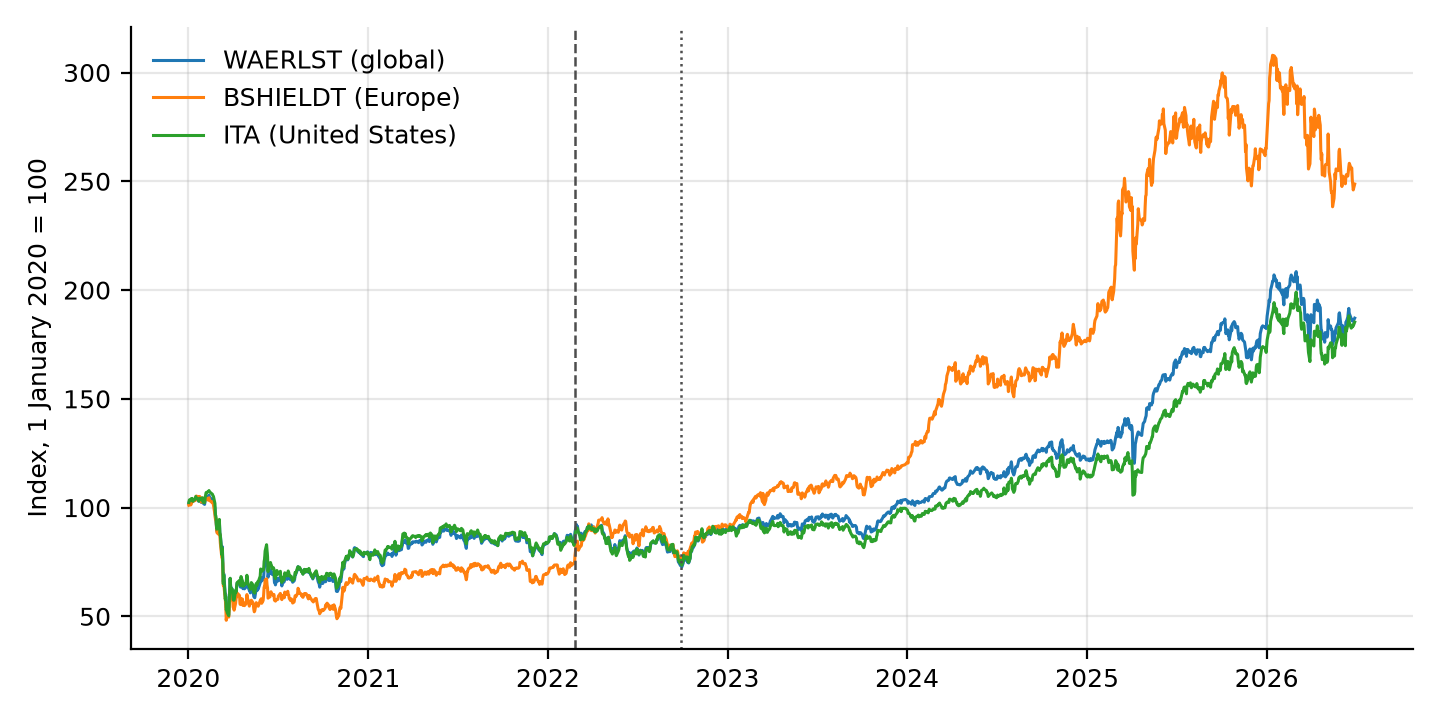
\includegraphics[width=1\textwidth]{fig1_defense_indices.png}
\caption{Defense-equity outcomes over time. WAERLST, BSHIELDT, and ITA are normalized to 100 on 1 January 2020. The dashed vertical line marks Russia's full-scale invasion of Ukraine on 24 February 2022. The dotted vertical line marks the beginning of the measured attack window on 29 September 2022.}
\label{fig:defense_indices}
\end{figure}

Figure~\ref{fig:attacks_news} combines the two war-information layers. The upper panel shows weekly Russian weapons launched against Ukraine, the middle panel shows conflict-related attention as a share of each source group's own output, and the lower panel shows average tone by source group. The figure illustrates that physical attack intensity and media attention are related but not identical: attack intensity rises steadily through 2025 and 2026 while attention settles well below its 2022 peak, and tone differs across Ukrainian, Russian state, Russian independent, and Western sources.

\begin{figure}[H]
\centering
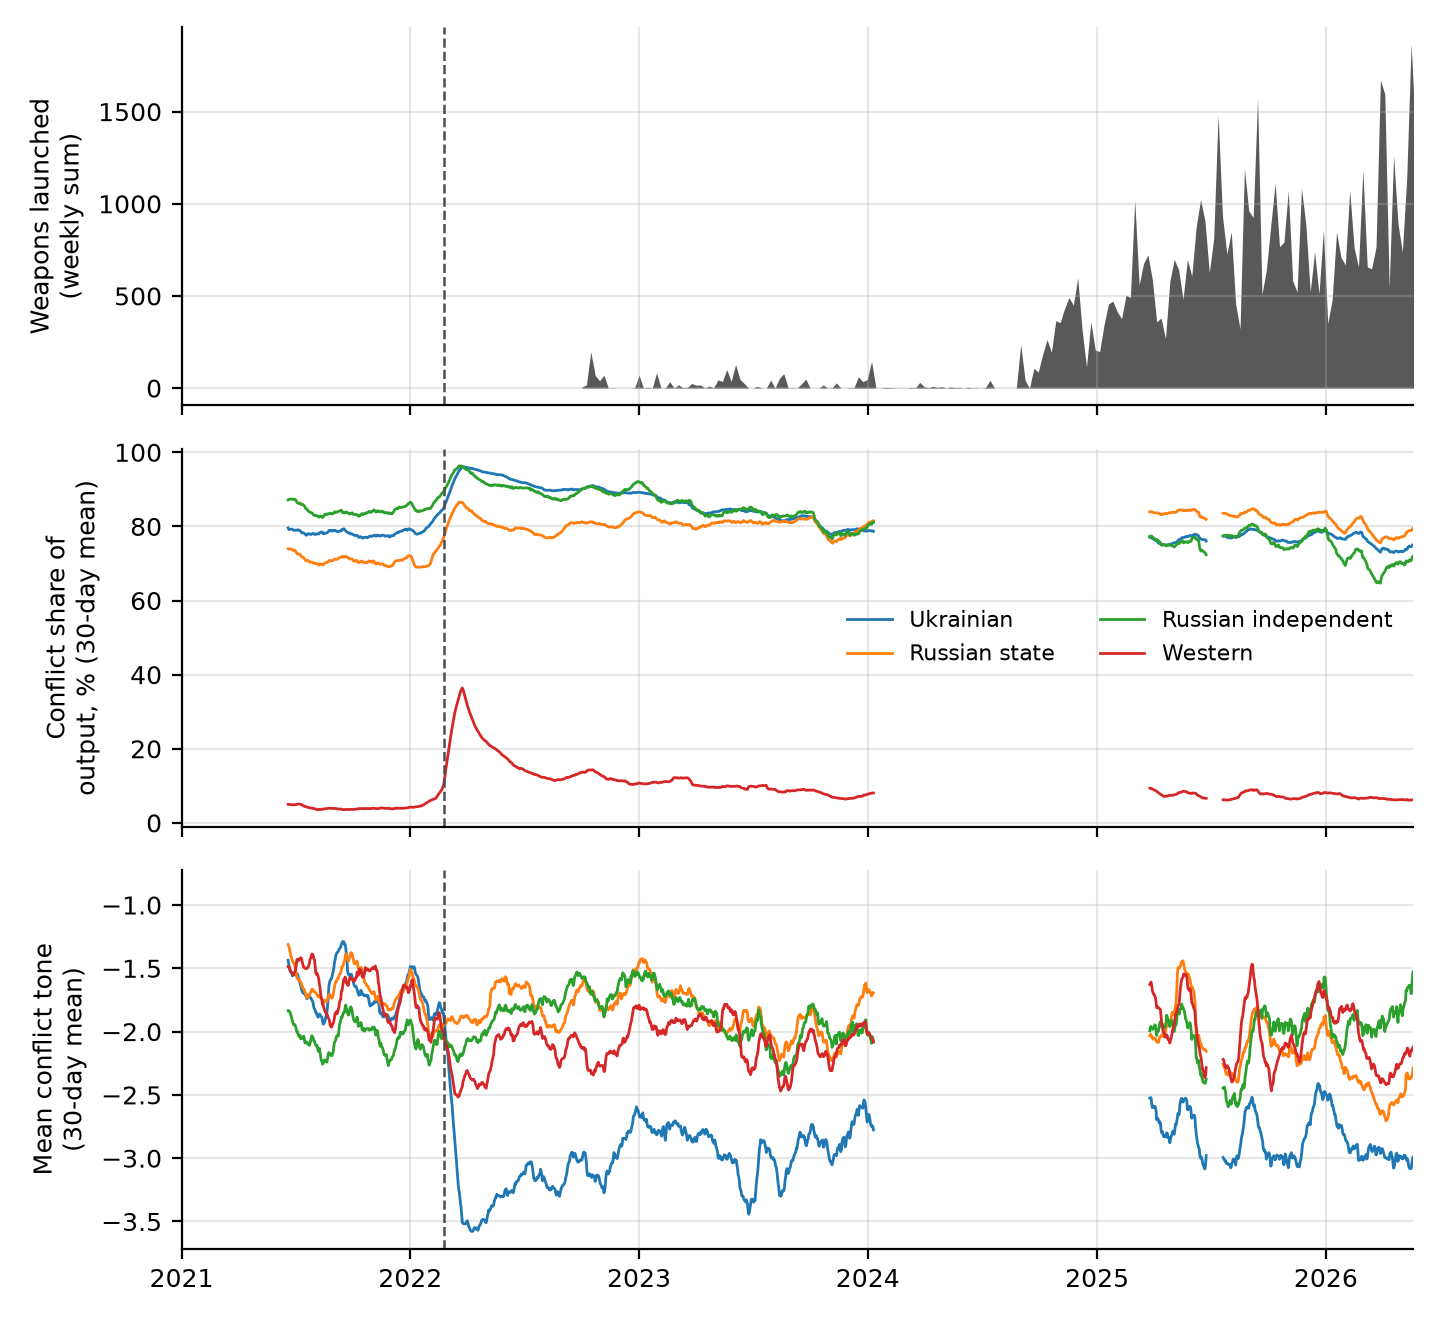
\includegraphics[width=1\textwidth]{fig2_attacks_news.png}
\caption{Physical attack intensity and multilingual news narratives. The first panel reports the weekly sum of Russian weapons launched. The second panel reports conflict-related articles as a share of each source group's own daily output, as a thirty-day mean. The third panel reports average GDELT tone for the same groups, where lower values indicate more negative language. Breaks in the lower two panels are days absent from the news archive and are left as breaks rather than interpolated.}
\label{fig:attacks_news}
\end{figure}

\section{Empirical Findings, Interpretation, and Implications}

\subsection{Forecasting Comparisons}

The empirical findings are organized around information-set comparisons rather than individual coefficients. This is important because the research question asks whether physical and narrative war signals improve forecasts, not whether one isolated coefficient is statistically significant in one specification. The main comparison is therefore between the financial baseline and the larger information sets P, N, PN, and PNG.

The first outcome is return predictability. Daily return prediction is difficult, and the prior from the equity-prediction literature is that out-of-sample improvements may be small \citep{goyal2008equity}. If attack or news variables reduce forecast error for WAERLST returns, this would be meaningful because it would show that war-specific information adds value beyond standard financial controls. If they do not reduce forecast error, the result would still be informative because it would suggest that daily defense-equity returns incorporate such information quickly or that the signals are too noisy at the daily horizon.

The second outcome is volatility predictability. The prior is stronger for volatility than for returns because geopolitical shocks may change uncertainty even if they do not predict the sign of returns. For that reason, the volatility results may provide the more natural test of whether physical attacks and news narratives matter for financial risk. The main volatility comparison should focus on QLIKE and on whether attack-enhanced or news-enhanced models improve over financial-only GARCH-family benchmarks.

\begin{table}[H]
\centering
\caption{Out-of-sample return forecast performance}
\label{tab:return_forecasts}
\begin{threeparttable}
\begin{tabular}{llrrrrrr}
\toprule
Model & Information set & Horizon & MAE & RMSE & Dir.\ acc. & $R^2_{OS}$ & CW $p$ \\
\midrule
Historical mean & F & 1 & 1.073 & 1.375 & 0.503 & 0.000 & --- \\
AR(1) & F & 1 & 1.083 & 1.380 & 0.483 & -0.007 & 0.542 \\
Ridge & F & 1 & 1.088 & 1.432 & 0.462 & -0.086 & 0.512 \\
XGBoost & F & 1 & 1.092 & 1.408 & 0.483 & -0.049 & 0.183 \\
XGBoost & P & 1 & 1.062 & 1.357 & 0.510 & 0.025 & 0.013 \\
XGBoost & N & 1 & 1.076 & 1.381 & 0.462 & -0.009 & 0.059 \\
XGBoost & PN & 1 & 1.053 & 1.345 & 0.497 & 0.043 & 0.006 \\
XGBoost & PNG & 1 & 1.066 & 1.369 & 0.503 & 0.008 & 0.025 \\
\addlinespace
Historical mean & F & 5 & 2.541 & 3.155 & 0.455 & 0.000 & --- \\
AR(1) & F & 5 & 2.548 & 3.158 & 0.448 & -0.002 & 0.517 \\
Ridge & F & 5 & 2.609 & 3.324 & 0.469 & -0.111 & 0.189 \\
XGBoost & F & 5 & 2.805 & 3.477 & 0.476 & -0.215 & 0.121 \\
XGBoost & P & 5 & 2.649 & 3.232 & 0.503 & -0.050 & 0.072 \\
XGBoost & N & 5 & 2.807 & 3.424 & 0.448 & -0.178 & 0.149 \\
XGBoost & PN & 5 & 2.636 & 3.185 & 0.483 & -0.019 & 0.069 \\
XGBoost & PNG & 5 & 2.688 & 3.267 & 0.435 & -0.072 & 0.120 \\
\bottomrule
\end{tabular}
\begin{tablenotes}
\small
\item Notes: The table reports WAERLST out-of-sample forecasts on the measured sample. MAE and RMSE are in return percentage points. Directional accuracy is the share of dates on which the predicted and realized return have the same sign. $R^2_{OS}$ is the Campbell--Thompson out-of-sample $R^2$ against the historical-mean benchmark, and CW $p$ is the Clark--West $p$-value for that comparison, which is the appropriate test because every specification nests the benchmark. Both horizons use 145 forecast dates. F is the financial baseline, P adds physical attack variables, N adds news variables, PN combines physical and news variables, and PNG adds narrative gaps. No specification in this table survives false-discovery-rate correction across the full grid.
\end{tablenotes}
\end{threeparttable}
\end{table}

Table~\ref{tab:return_forecasts} shows that the return-forecast evidence is weak. At the one-day horizon three war-augmented specifications improve on the historical mean, the best of them by 1.8 percent in MAE. At the five-day horizon the historical mean is the best model outright and every war-augmented specification is worse. The improvements at one day are small in absolute terms, and none survives the false-discovery-rate correction applied across the full grid.

Across the whole design, which spans three outcomes, two horizons, two samples, and five information sets in 144 specifications, 16 produce a positive out-of-sample $R^2$, 23 have a nominal Clark--West $p$-value below 0.05, and none survives correction at a 5 percent false-discovery rate. Models that use no war variables at all win eight of the twelve outcome-horizon-sample cells. The main interpretation is therefore not that war signals predict returns, but that the daily attack and news variables do not robustly improve return forecasts beyond financial information.

\begin{figure}[H]
\centering
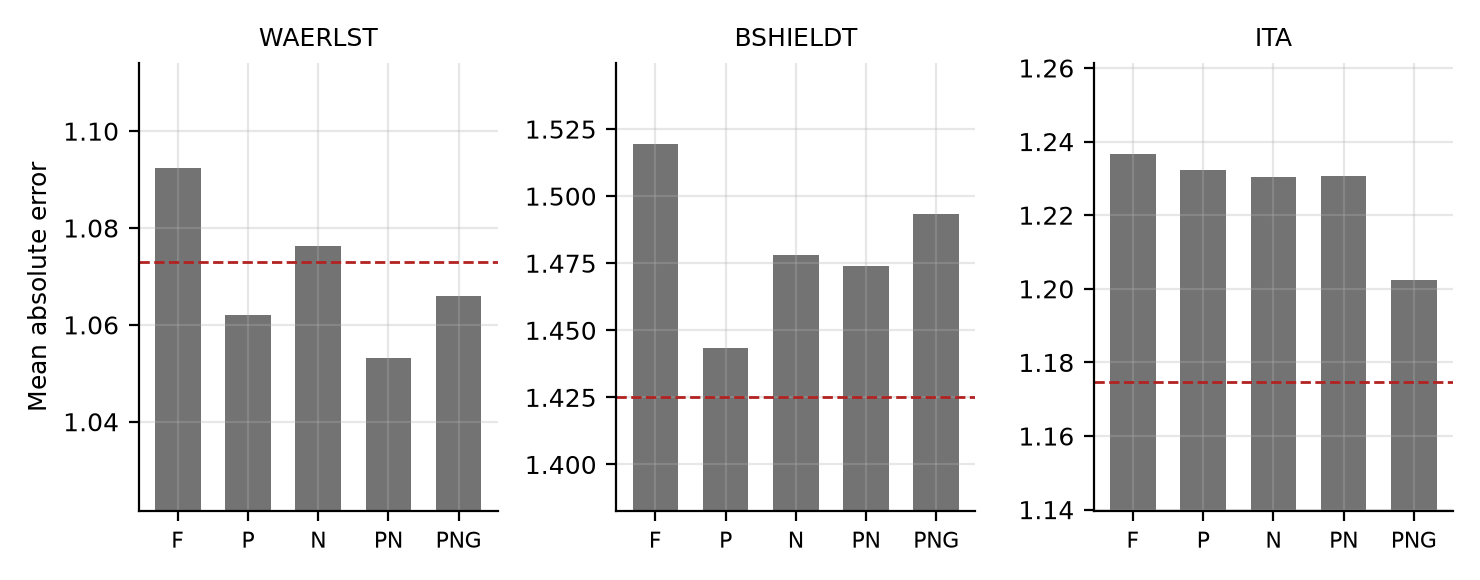
\includegraphics[width=1\textwidth]{fig3_return_mae_infosets.png}
\caption{One-day return forecast error by XGBoost information set. Bars report mean absolute error for XGBoost models using financial controls only (F), physical attacks (P), news variables (N), physical plus news variables (PN), and physical plus news plus narrative gaps (PNG). The dashed horizontal line is the historical-mean benchmark for each outcome.}
\label{fig:return_mae_infosets}
\end{figure}

\begin{table}[H]
\centering
\caption{Out-of-sample volatility forecast performance}
\label{tab:volatility_forecasts}
\begin{threeparttable}
\begin{tabular}{lrrrr}
\toprule
Model & Horizon & QLIKE & MAE & RMSE \\
\midrule
EGARCH & 1 & 1.380 & 1.613 & 2.775 \\
GJR-GARCH & 1 & 1.405 & 1.613 & 2.786 \\
GARCH & 1 & 1.425 & 1.596 & 2.798 \\
HAR-RV & 1 & 3.795 & 1.479 & 3.093 \\
HAR-RV-X (P) & 1 & 3.651 & 1.495 & 3.017 \\
HAR-RV-X (N) & 1 & 4.378 & 1.474 & 3.084 \\
HAR-RV-X (PNG) & 1 & 4.446 & 1.530 & 3.045 \\
\addlinespace
HAR-RV & 5 & 0.171 & 2.282 & 3.910 \\
HAR-RV-X (P) & 5 & 0.176 & 2.418 & 4.110 \\
HAR-RV-X (N) & 5 & 0.172 & 2.331 & 3.940 \\
HAR-RV-X (PNG) & 5 & 0.175 & 2.582 & 4.369 \\
GJR-GARCH & 5 & 0.335 & 4.539 & 6.885 \\
GARCH & 5 & 0.352 & 4.535 & 6.985 \\
EGARCH & 5 & 0.489 & 5.125 & 7.756 \\
\bottomrule
\end{tabular}
\begin{tablenotes}
\small
\item Notes: The table reports WAERLST volatility forecasts on the measured sample, ordered by QLIKE within each horizon. The volatility target is a return-based realized-variance proxy because intraday prices are not available. QLIKE is the main volatility loss. Horizon 1 uses 233 forecast dates and horizon 5 uses 232. HAR-RV is the heterogeneous-autoregressive benchmark and HAR-RV-X adds the indicated war block to it.
\end{tablenotes}
\end{threeparttable}
\end{table}

Table~\ref{tab:volatility_forecasts} shows that the GARCH family provides the strongest benchmarks at the one-day horizon under QLIKE, with EGARCH the best single model, while the heterogeneous-autoregressive specifications are stronger at five days. Adding war variables does not improve on the relevant benchmark at either horizon. Some augmented specifications have a lower mean absolute error than the benchmark, but QLIKE is the preferred volatility loss precisely because squared-error criteria on a variance are dominated by a small number of extreme days.

Across all 48 war-augmented volatility specifications, four have a lower QLIKE than the HAR-RV benchmark, none of those differences is statistically significant, and eight augmented specifications are significantly worse. Every specification that survives the false-discovery-rate correction is a deterioration rather than an improvement. The volatility evidence therefore does not support a robust incremental role for attack and news variables.

This is the more demanding of the two tests, and it is worth saying why. Daily returns are close to unforecastable in general, so failing to predict them is the default outcome and weak evidence about the information content of a signal. Volatility is different: it clusters, it persists, and standard models forecast it with some success. It is also where geopolitical shocks would be expected to appear, since an attack wave may plausibly change uncertainty even when its direction for prices is ambiguous. A war signal that does not improve a volatility forecast has failed on favorable ground.

\subsection{Machine-Learning Interpretation}
\label{sec:mlinterp}

The XGBoost results are useful mainly as a nonlinear robustness check. If the war-specific variables contained strong nonlinear predictive information, the tree model should have been able to exploit it more easily than ridge regression. The results show a partial version of this pattern and no more. At the one-day horizon the war-augmented XGBoost specifications do improve on the historical mean for WAERLST, and the corresponding ridge specifications do not, which is consistent with any usable structure being nonlinear rather than linear. But the improvements are small, they do not survive correction across the grid, and they reverse at the five-day horizon, where the historical mean is best and every extended specification is worse. For BSHIELDT the AR(1) benchmark dominates at both horizons. This pattern argues against a strong machine-learning forecasting result.

A forecast comparison answers whether a block of variables improves prediction. It does not answer a prior and more direct question about the same model: how much of the weight it places on its inputs goes to war variables at all. A model that never looked at the attack and news blocks would produce the same null as a model that looked hard and found nothing, and the two would mean different things. The fitted model is therefore decomposed by TreeSHAP, which splits each prediction exactly into per-feature contributions, averaged in absolute value over the held-out period so that a variable pushing forecasts up as often as down still registers.

\begin{figure}[H]
\centering
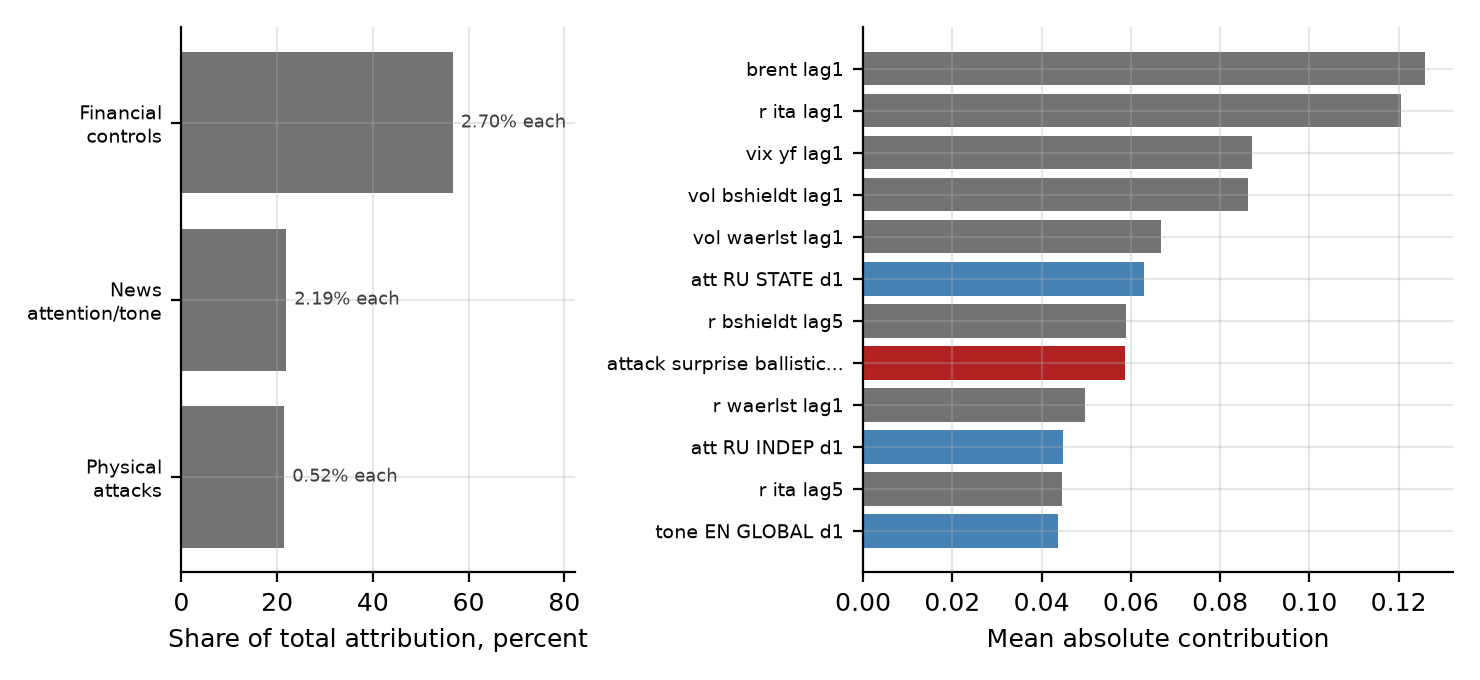
\includegraphics[width=1\textwidth]{fig4_shap_attribution.png}
\caption{Attribution of the fitted model across variable blocks. The left panel reports each block's share of total absolute contribution, annotated with the average per predictor in that block. The right panel reports the twelve largest individual contributions, colored by block: grey for financial controls, blue for news variables, red for physical attack variables. The model is the physical-plus-news specification for one-day WAERLST returns, decomposed over the held-out period.}
\label{fig:shap}
\end{figure}

Figure~\ref{fig:shap} shows that the model is not ignoring the war variables. They receive 43.3 percent of its total attribution: 21.9 percent to news attention and tone, and 21.5 percent to physical attacks. The single largest contribution from outside the financial block is the change in Russian state media's conflict attention, which ranks sixth of the seventy-two predictors, and a ballistic-missile attack-surprise measure ranks eighth.

That is the more interesting version of the null. The model had the war variables, used them substantially, and still did not beat a historical mean by a margin that survives correction. Attribution measures how much a fitted model relies on a variable, not whether that reliance helps out of sample; a tree that splits on noise attributes weight to that noise. The forecast comparison and the attribution are therefore consistent rather than contradictory, and together they say something the forecast comparison alone cannot: the failure is not one of attention.

The per-predictor figures qualify this in a way the totals conceal. The physical block reaches its 21.5 percent share across 41 predictors, an average of 0.52 percent each, while the 21 financial controls average 2.70 percent and the 10 news variables 2.19 percent. Measured per variable, physical attack measures are the weakest of the three blocks by a factor of four or five. The block accumulates attribution largely by being large.

Two cautions belong with this reading. The model being decomposed does not beat its benchmark by a detectable margin, so the ranking of individual variables inside a block should not be over-interpreted; it is the comparison across blocks that carries the argument. And attribution is computed on one specification --- the physical-plus-news set for one-day WAERLST returns --- chosen because it is the best-performing extended specification in Table~\ref{tab:return_forecasts}, which makes it the most favourable case for the war variables rather than a representative one.

\subsection{Robustness and Interpretation}

Robustness checks use ITA and BSHIELDT to test whether the results depend on the geographic scope of the defense-equity outcome. ITA checks whether the global WAERLST result also appears in a U.S. traded aerospace and defense ETF. BSHIELDT checks whether the result is stronger in Europe, where the economic and political relevance of the Russia--Ukraine war may be more direct.

\begin{table}[H]
\centering
\caption{Robustness checks across defense-equity outcomes and samples}
\label{tab:robustness}

\begin{threeparttable}
\small
\setlength{\tabcolsep}{4pt}

\begin{tabularx}{\textwidth}{
    @{}
    l
    c
    c
    c
    >{\raggedright\arraybackslash}X
    @{}
}
\toprule
Outcome & Best baseline loss & Best extended loss & Improvement & Interpretation \\
\midrule
\multicolumn{5}{@{}l}{\emph{Full sample, 2015--2026}} \\
WAERLST, h=1  & 0.937 & 0.931 & 0.6\%  & Small gain, not significant \\
WAERLST, h=5  & 2.211 & 2.308 & -4.4\% & Historical mean dominates \\
BSHIELDT, h=1 & 1.335 & 1.351 & -1.2\% & No European return gain \\
BSHIELDT, h=5 & 2.933 & 3.066 & -4.5\% & AR(1) baseline dominates \\
ITA, h=1      & 1.041 & 1.063 & -2.1\% & No U.S. ETF gain \\
ITA, h=5      & 2.264 & 2.196 & 3.0\%  & Small gain, not significant \\
\addlinespace
WAERLST, h=1  & 1.073 & 1.053 & 1.8\%  & Small gain, not significant \\
WAERLST, h=5  & 2.541 & 2.629 & -3.5\% & Historical mean dominates \\
BSHIELDT, h=1 & 1.413 & 1.411 & 0.2\%  & Small gain, not significant \\
BSHIELDT, h=5 & 3.232 & 3.302 & -2.2\% & AR(1) baseline dominates \\
ITA, h=1      & 1.175 & 1.202 & -2.3\% & No U.S. ETF gain \\
ITA, h=5      & 2.603 & 2.588 & 0.6\%  & Small gain, not significant \\
\bottomrule
\end{tabularx}

\begin{tablenotes}
\small
\item Notes: Loss is MAE in return percentage points. The best baseline is
the best model that does not use attack or news variables, including the
historical mean, AR(1), and models estimated on the financial set alone. The
best extended loss is the best model using P, N, PN, or PNG. Positive
improvement means lower MAE than the baseline. The second block restricts the
sample to the measured attack window beginning 29 September 2022. No extended
specification in this table survives false-discovery-rate correction across the
grid.
\end{tablenotes}

\end{threeparttable}
\end{table}

The robustness evidence confirms the conservative interpretation. A war-augmented information set achieves a lower MAE than every baseline in five of the twelve cells, by between 0.2 and 3.0 percent, and is worse in the other seven. The gains are concentrated at the one-day horizon and reverse at five days, and none is statistically distinguishable from zero once the size of the specification grid is taken into account. Read together with Table~\ref{tab:return_forecasts}, the picture is one of small and unstable differences around a benchmark rather than a detectable signal.

A further check addresses the sample restriction itself. The comparison above drops the 149 days for which physical data does not exist, so that every information set is judged on identical observations. That is right for comparing sets and wrong for one question, because a model using only news requires no physical data and the exclusion denies it precisely the months in which the war began. Estimated on its own, with those days retained and the physical block dropped, the news set has 904 observations against 579 on the measured sample --- more than half as many again, and including 143 days inside the invasion window.

Over that longer sample the news set does not improve on the historical mean in any of the twelve specifications it supports. Every out-of-sample $R^2$ is negative, ranging from $-0.04$ to $-0.20$, and no Clark--West comparison survives correction. The conclusion does not depend on the sample restriction that the attack data imposes.

It is worth being explicit about what limits that sample, because it is not the news. The extraction runs from February 2015, but the defence-equity indices begin in January 2020, so a forecasting model cannot reach further back than its target does however long the news series is. The gain from the longer news sample is therefore real but bounded, and the binding constraint on this design is the availability of the financial outcome rather than of the war signal.

The two samples also answer a question about the pre-war period directly. Carrying those years as zeros in the physical block does not change the verdict, and it does not help the physical layer: mean out-of-sample $R^2$ for the news set improves slightly on the longer sample, by 0.013, while the physical, combined, and narrative-gap sets all deteriorate, by between 0.025 and 0.035. The reason is straightforward. In 1,757 of the added trading days every physical variable is identically zero, so those observations add sample size without adding variation in the quantity whose predictive content is being tested. The assumption is defensible, and it is not free.

\section{Conclusion}

This thesis asks whether physical Russian air-attack intensity and multilingual news narratives improve out-of-sample forecasts of defense-equity returns and volatility. The analysis combines official Bloomberg defense-equity indices, daily physical attack data, and GDELT news variables while enforcing timing rules designed to prevent look-ahead bias. The research design is predictive rather than causal: it evaluates whether information available before the forecast date improves forecast accuracy.

The main contribution is to compare physical and narrative war signals in the same forecasting framework. The physical layer measures realized military intensity through weapons launched, weapons destroyed, interception rates, weapon composition, and attack-surprise variables. The narrative layer measures news attention, tone, and differences in tone across Ukrainian, Russian state, Russian independent, Western, and native-English source groups. This distinction is useful because the market may respond differently to what happens physically and to how those events are reported. Classifying sources by publisher rather than by subject is what makes the second half of that comparison meaningful, and the classifier is validated externally, audited domain by domain, and re-estimated under alternative rules so that the news result does not rest on one set of unexamined choices.

The final answer to the research question is cautious. Physical air-attack intensity and multilingual news narratives do not provide robust incremental out-of-sample predictive power for defense-equity returns or volatility in this sample. Across 144 return specifications, 16 improve on the historical mean and none survives a false-discovery-rate correction, while models using no war variables win two-thirds of the outcome-horizon cells. The one-day WAERLST results show small improvements from the combined physical-and-news set, but they are not statistically distinguishable from zero and they reverse at the five-day horizon. For volatility, standard GARCH-family benchmarks are not improved upon by war-augmented specifications under QLIKE, and every statistically detectable difference runs the wrong way. The evidence therefore supports a null or near-null conclusion rather than a strong predictability result.

The thesis has several limitations. First, the analysis does not identify causal effects of attacks or news on defense-equity prices. Second, the daily frequency may be too coarse for some market reactions and too noisy for others; intraday data would allow a cleaner analysis of immediate price discovery. Third, volatility is measured using close-to-close returns rather than high-frequency realized volatility. Fourth, GDELT tone remains an imperfect proxy for media narratives: the source classification is validated externally at the level of the publishing domain, but that validation cannot establish that GDELT has attributed every article to the right domain in the first place, which only a reader with the relevant languages could check. Fifth, physical attack data exist only from late September 2022, so the months of the invasion itself lie outside every specification that uses them, and the number of out-of-sample forecast observations remains modest.

Several extensions are possible. Future work could use intraday financial data to study whether attack announcements or major news releases are incorporated within hours rather than days. A second extension would use point-in-time index constituents to study firm-level heterogeneity by country, product type, or exposure to government procurement. A third extension would apply multilingual transformer models to article text, which could measure narrative content more directly than GDELT tone. A final extension would compare the Russia--Ukraine war with other geopolitical conflicts to test whether defense-equity predictability is conflict-specific or more general.

The contribution of this thesis is therefore narrow but evidence-based. It does not find strong incremental predictability from daily physical attacks or multilingual news narratives, but it shows this through a transparent dataset, a careful timing design, a source classification that is validated rather than assumed, and an out-of-sample comparison of physical and narrative war information in which the size of the specification grid is accounted for. The study contributes to the literature by testing a clear forecasting question in a setting where geopolitical risk, news, and defense-equity markets meet.

\newpage
\appendix
\section{Additional Diagnostic Figures}

\begin{figure}[H]
\centering
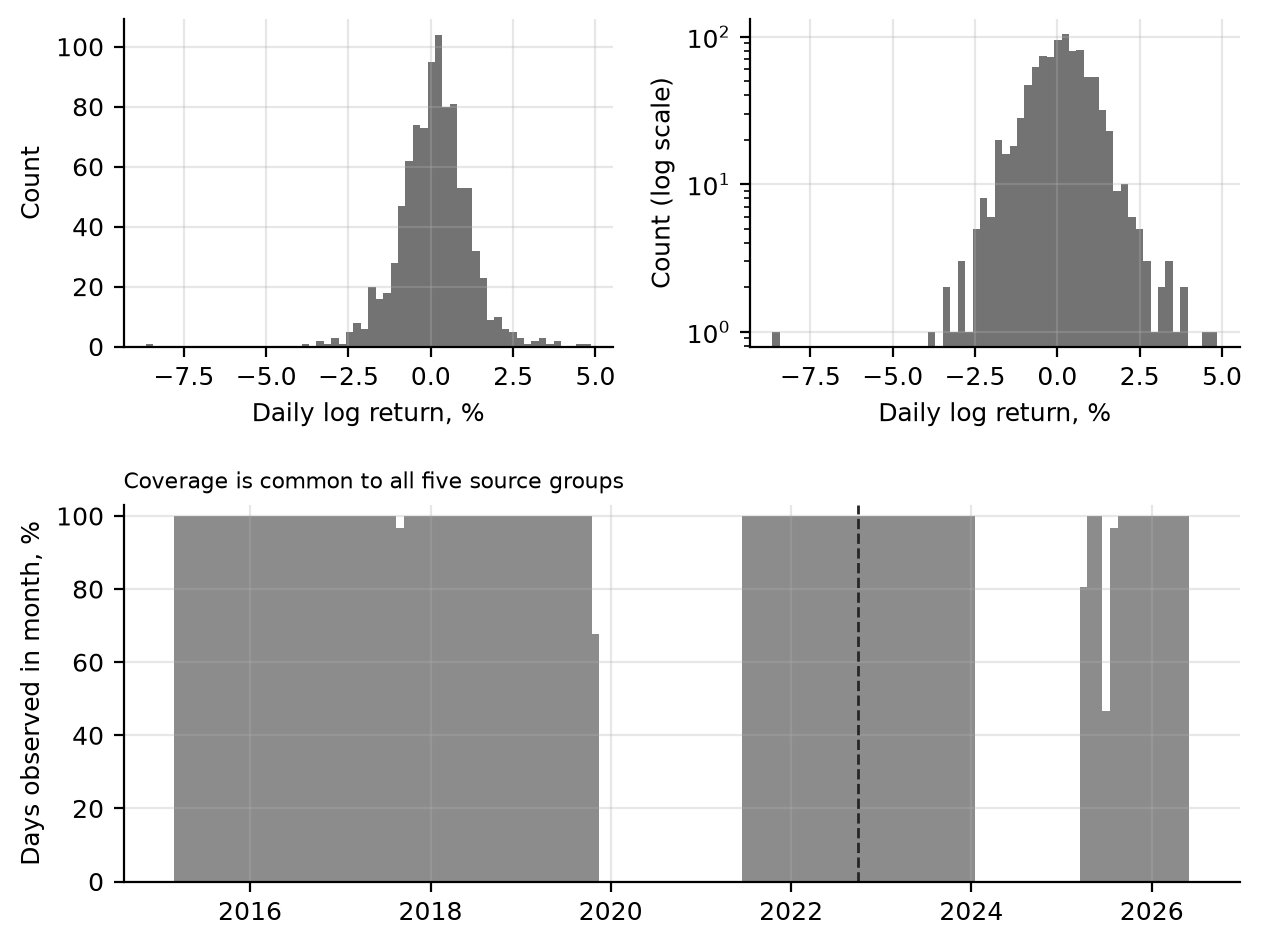
\includegraphics[width=1\textwidth]{figA1_diagnostics.png}
\caption{Diagnostics for the forecasting target and the news sample. The upper panels report the distribution of the one-day WAERLST return target, on a linear count axis and on a logarithmic one that makes the tails easier to see. The lower panel reports monthly coverage of the news extraction, as the share of days in each month for which the series are observed; coverage is common to all five source groups, since they are derived from the same extraction. The dashed vertical line marks the beginning of the measured attack window on 29 September 2022.}
\label{fig:appendix_diagnostics}
\end{figure}

\newpage

\newpage
\bibliography{references}

\end{document}
